\documentclass[11pt,fleqn]{book} %taille de la police par défaut, et équations jusitifées à gauche
\usepackage[top=3cm,bottom=3cm,left=3.2cm,right=3.2cm,headsep=10pt,a4paper]{geometry} % marges
\usepackage{xcolor}
\definecolor{enstabGreen}{HTML}{C8D200} 	%vert  	#c8d200 
\definecolor{enstabLightGreen}{HTML}{E9ED99} 	%vert  	#c8d200 
\definecolor{enstabLightBlue}{HTML}{009EE0} %bleu clair 	#009ee0
\definecolor{enstabVeryLightBlue}{HTML}{99D8F3} %bleu clair 	#009ee0
\definecolor{enstabDarkBlue}{HTML}{005C8F}	%bleu foncé 	#005c8f
\definecolor{enstabDarkGrey}{HTML}{333333}	%gris fort 	#333333
\definecolor{enstabLightGrey}{RGB}{48,48,48}	%gris fort 	#333333
\definecolor{enstabParme}{HTML}{8878B2}		%parme 	#8878b2
\definecolor{enstabOrange}{HTML}{F18E00} 	%orange 	#f18e00
\usepackage[colorlinks=true,
        urlcolor=enstabLightBlue,
        anchorcolor=enstabDarkBlue,
        linkcolor=enstabDarkBlue,
        citecolor=enstabDarkGrey,
        pdfauthor={Johan B. C. Engelen},
        pdfkeywords={SVG; LaTeX; Inkscape},
        pdftitle={How to include an SVG image in LaTeX},
        pdfsubject={Describes how to include an SVG image easily in LaTeX using Inkscape}] {hyperref}
\usepackage{url}
\usepackage[utf8]{inputenc} % lettres accentuées
\usepackage[T1]{fontenc}    % Use 8-bit encoding that has 256 glyphs
\usepackage[frenchb]{babel} % Pour le français
\usepackage{cclicenses}     % Licences CC
\usepackage{epigraph}
\usepackage{eso-pic}        % pour une image en fond, page de titre
\usepackage{graphicx}       % Pour inclure des images
\graphicspath{{images/}}    % Où sont les images ?

\usepackage{booktabs}       % pour de jolis tableaux
\usepackage{fancyhdr}       % pour des entêtes et pieds de pages améliorés.
\usepackage{makeidx}        % requis pour faire les index
\usepackage[toc]{glossaries} %requis pour faire le glossaire % Tous les packages nécessaires à la compitlation

\makeindex           % donne l'ordre de créer l'index
\newacronym{IS}{IS}{Ingénierie Système}
\newacronym{WBS}{WBS}{Work Breakdown Structure}
\makeglossaries      % donne l'ordre de créer le glossaire

\begin{document}
\renewcommand{\bibname}{Références bibliographiques}  % des jolis noms pour les sections bibliographiques
\renewcommand{\glossaryname}{Glossaire}               % et glossaire

%----------------------------------------------------------------------------------------
%	 PAGE DE TITRE
%----------------------------------------------------------------------------------------

\begingroup
\thispagestyle{empty}
\AddToShipoutPicture*{\put(6,5){
\includegraphics[scale=1]{FondTitre}}} % Image background
\begin{center}
\vspace*{3cm}
{\Huge \textsc{\textbf{Rapport d'avancement}}}\\
\vspace*{1cm}
{\Huge \textbf{PSPID}}\par % ACRONYME du projet
\vspace*{1cm}
{\huge Projet exemplaire à plus d'un titre}\par % Intitulé du projet
\end{center}
\vspace*{6cm}

\hspace*{6cm}
\textbf{\huge rédigé par :} 
\begin{flushright}
{
\huge
Jojo Lafritte\\
Zaza Lasalade\\
Gudule Lembrouille\\
 Gaston Letelelefon\\
}
\end{flushright}
\vspace*{1cm}
\hspace*{6cm}
{\huge \textbf{sous la direction de :}}\\
\begin{flushright}
{\huge
Olivier Reynet\\
}
\end{flushright}
\endgroup


%----------------------------------------------------------------------------------------
%	COPYRIGHT PAGE
%----------------------------------------------------------------------------------------
\newpage
~\vfill
\thispagestyle{empty}

\noindent \bysa 2014 Olivier Reynet\\ % Copyright notice

%\noindent \textsc{Published by Publisher}\\ % Publisher

%\noindent \textsc{book-website.com}\\ % URL

\noindent Licensed under the Creative Commons Attribution-ShareAlike 4.0 International Public License.\\ % License information

\noindent \textit{Première impression, juillet 2014} % Printing/edition date

%----------------------------------------------------------------------------------------
%	SOMMAIRE
%----------------------------------------------------------------------------------------

\pagestyle{empty} % enlever les entêtes pour le sommaire
\tableofcontents  % Imprime le sommaire
\cleardoublepage  % pour commencer sur une page impaire

\frontmatter   % La partie non numérotée préalable au document principal


\chapter{Remerciements}
\epigraph{La gratitude est non seulement la plus grande des vertus, mais c'est également la mère de tous les autres.}{Emil Cioran}

Je tiens à remercier tous les contributeurs de \LaTeX qui nous permettent aujourd'hui de produire des documents de qualité professionnelle sans avoir à se préoccuper de son apparence : des livres, des articles, des mémentos dans presque toutes les langues, mais aussi de la musique et des dessins. Ce logiciel ne connaît pas de limites.
 

\chapter{Préambule}
\epigraph{Le chemin est long du projet à la chose.}{Molière}

\section{Compilation du document}

Un document \LaTeX peut se compiler au travers d'un IDE (TexSutdio, TeXMaker par exemple).
Le répertoire de ce document contient également un Makefile qui permet de compiler simplement en ligne de commande. 
La fabrication du glossaire et de l'index est prise en charge dans ce Makefile. 

\section{Références internes}

Les références internes sont des renvois vers des figures, des tableaux ou des sections du rapport.
\LaTeX introduit un mécanisme simple pour établir ce genre de référence, via les commandes  \textsf{\textbackslash label} et \textsf{\textbackslash ref}. 
La première sert à définir une ancre dans le document, la seconde à la citer.
Voici par exemple une référence interne vers la section intitulée \textit{Approche Top-Down} (cf. section  \ref{sec:top-down}).
Les figures  et les tableaux  sont référencés de la même la manière (cf. figure \ref{fig:gomboc} et tableau \ref{tab:exemple}). \index{Table} \index{Figure}

\begin{table}[h]
\centering
\begin{tabular}{lll}
\toprule
\textbf{Algorithmes} & \textbf{Performance (s)} & \textbf{Gain (dB)}\\
\midrule
Algorithme 1 & 0.0003262 & 0.562 \\
Algorithme 2 & 0.0015681 & 0.910 \\
Algorithme 3 & 0.0009271 & 0.296 \\
\bottomrule
\end{tabular}
\caption{\label{tab:exemple}Performances et gains des algorithmes envisagés.}
\end{table}

\begin{figure}[h]
\centering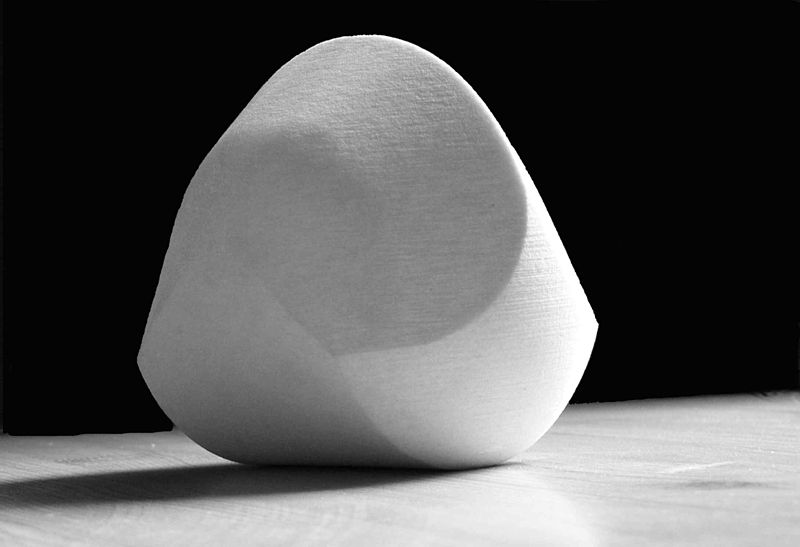
\includegraphics[scale=0.25]{Gomboc.jpg}
\caption{\label{fig:gomboc}Gömböc : un objet homogène tridimensionnel mono-monostatique. (source : Wikipedia)}
\end{figure}


Pour insérer des entrées dans l'index, il suffit de déclarer des mots via la commande \textsf{\textbackslash index} comme suit\footnote{Évidemment, elle n'est pas visible dans le document pdf\dots Faites un tour à la fin du document !}. \index{Contexte du projet}

Pour utiliser le glossaire, il faut définir les termes dans le fichier \textsf{glossaire.tex} en utilisant la commande \textsf{\textbackslash newacronym\{label\}\{abbrv\}\{full\}}. 
Puis,  \textsf{\textbackslash gls\{label\}} permet de les utiliser dans le document. 


Par exemple, les UVs 3.4 et 4.4 sont une initiation à l'\gls{IS}.


\section{Références externes}

Les références externes sont des documents numériques, des livres, des articles, des images ou des vidéos qui ne sont pas présents dans le rapport. 
\LaTeX propose un mécanisme simple de citation.
Pour plus de détails, vous pouvez consulter les références suivantes \cite{maguis2010redigez,desgraupes2003latex,bitouze2010latex} qui sont présentent à la médiathèque de l'ENSTA Bretagne, ou celle-ci directement sur le web \cite{openclassroomLaTeX}.  

Pour citer des documents, il suffit d'appeler la commande \textsf{\textbackslash cite\{key\}} ainsi \cite{lamport1985i1}. 
La clé de citation est celle qui référence l'ouvrage dans le fichier de bibliographie intitulé   \textsf{bibliographie.bib}.
Ce fichier d'exemple contient tous les types de documents dont vous aurez besoin : livre, article de journal, références web,  rapport\dots 
Une fois insérée et compilée, la citation devient un lien dans le fichier pdf, redirigeant ainsi directement vers le détail de l'ouvrage cité dans la bibliographie située à la fin du document.
 


\mainmatter       % La partie principale du document
\pagestyle{fancy} % Pour afficher les entêtes

%----------------------------------------------------------------------------------------
%	PART I 
%----------------------------------------------------------------------------------------
\part{Définition du projet}
\chapter{Formulation initiale du projet}


\section{Contexte}

Pour citer des documents, il suffit d'appeler la référence ainsi \cite{article}.


\section{Expression initiale du besoin}
\chapter{État de l'art}

Quel est l’existant ? 

Quelles sont les solutions connues (algorithmes, matériels, logiciels, comportements, stratégies) ? 

Que pourrait-on (ré)utiliser pour le projet ? 

%----------------------------------------------------------------------------------------
%	PART II 
%----------------------------------------------------------------------------------------
\part{Dossier fonctionnel}
\chapter{Ingénierie des exigences}
\section{Approche Top-Down}
\label{sec:top-down}

\section{Approche Bottom-Up}

\section{Fonctions principales du système}

\chapter{Spécification fonctionnelle  3 axes}

\section{Raffinement FAST}
\section{Spécification des données}
\section{Spécification des comportements}


\chapter{Architecture fonctionnelle}




%----------------------------------------------------------------------------------------
%	PART III 
%----------------------------------------------------------------------------------------
%\part{Implémentation}
%
\chapter{Architecture physique}

%\chapter{Interfaces}
%\chapter{Structure de découpage du projet}

SDP en français, ou WBS Work Breakdown Structure en anglais 
%\chapter{Tests unitaires}

%----------------------------------------------------------------------------------------
%	PART IV 
%----------------------------------------------------------------------------------------
%\part{Intégration et validation}
%\chapter{Intégration}

%\chapter{Validation}

%----------------------------------------------------------------------------------------
%	PART V 
%----------------------------------------------------------------------------------------
\part{Organisation}
\chapter{Outils pour les échanges}

\chapter{Méthodes de travail}

\chapter{Répartition des tâches dans le temps}

%----------------------------------------------------------------------------------------
%	PART VI 
%----------------------------------------------------------------------------------------
\part{Choix, justifications et analyses du projet}

\chapter{Analyses}

\chapter{Regard critique}

\chapter{Et après ?}

\chapter{Conclusion}



\appendix
\part{Annexes}
\chapter{Première annexe}
\chapter{Deuxième annexe}
\chapter{Troisième annexe}

\backmatter % Partie finale du document, non numérotée

%----------------------------------------------------------------------------------------
%	BIBLIOGRAPHIE
%----------------------------------------------------------------------------------------
\addcontentsline{toc}{part}{Bibliographie}
\bibliographystyle{apalike-fr}
\bibliography{bibliographie.bib}
\nocite{*}

%----------------------------------------------------------------------------------------
%	INDEX
%----------------------------------------------------------------------------------------
\cleardoublepage
\phantomsection
\setlength{\columnsep}{0.75cm}
\addcontentsline{toc}{part}{Index}
\printindex

%----------------------------------------------------------------------------------------
%	GLOSSAIRE
%----------------------------------------------------------------------------------------
\cleardoublepage
\phantomsection
\setlength{\columnsep}{0.75cm}
\addcontentsline{toc}{part}{Glossaire}
\printglossaries

%----------------------------------------------------------------------------------------

\end{document}